%%=============================================================================
%% Methodologie
%%=============================================================================

\chapter{\IfLanguageName{dutch}{Methodologie}{Methodology}}%
\label{ch:methodologie}

% Door de vergaarde kennis uit de literatuurstudie in hoofdstuk \ref{ch:stand-van-zaken} over de mogelijke noden van scholieren met dyslexie, de complexiteit van wetenschappelijke artikelen, de technieken voor MTS en ATS, en de bijhorende valkuilen bij taalverwerking met AI, kunnen onderzoeksmethoden worden toegepast om een antwoord te vinden op de onderzoeksvraag. 

De vergaarde kennis uit de literatuurstudie dient als vertrekpunt voor het verdere onderzoek. Zo kan het de onderzoeksvraag beantwoorden met drie onderzoeksstappen. Eerst staat het onderzoek stil bij de nodige functionaliteiten om gepersonaliseerde ATS te kunnen verwezenlijken. Vervolgens achterhaalt het een geschikt taalmodel voor gepersonaliseerde ATS. Tot slot ontwikkelt het onderzoek Pentimentor, ofwel het prototype voor ATS van wetenschappelijke artikelen. Dit moet een eenduidige manier voor scholieren met dyslexie in de derde graad van het middelbaar onderwijs aanreiken om wetenschappelijke artikelen te vereenvoudigen. Zo doelt dit onderzoek om de haalbaarheid voor een toepassing voor gepersonaliseerde ATS te achterhalen met Pentimentor. 

\section{Requirementsanalyse}
\label{sec:requirementsanalyse}

Om het ontwikkelingsproces van Pentimentor gericht te sturen, moet het onderzoek bestaande en haalbare MTS en ATS-technologieën in bestaande tools nagaan. Zo gebeurt het verkennen en experimenteren op ATS-technieken bij beschikbare tools door een kwalitatief onderzoek in de vorm van een requirementsanalyse. Het resultaat van deze onderzoeksfase is een moscow-schema dat de benodigde en haalbare functionaliteiten voor een ATS-toepassing definieert. Met dit kan het onderzoek een vergelijkbare toepassing ontwikkelen voor gepersonaliseerde ATS van wetenschappelijke artikelen met de kwaliteiten van gepersonaliseerde MTS. Daarnaast achterhaalt deze fase de ontbrekende MTS-functionaliteiten die tabel \ref{table:benefits-mts} in de literatuurstudie uitwees. De geteste toepassingen, opgesomd in tabel \ref{table:shortlist-tools}, beschikken over (gepersonaliseerde) ATS-technieken. Deze lijst omvat erkende toepassingen van de overheid en toepassingen die leerkrachten of scholieren kunnen gebruiken om teksten te vereenvoudigen. Met deze onderzoeksmethode kan het onderzoek een antwoord geven op de volgende twee deelvragen van het onderzoek.

\begin{itemize}
	\item Welke functies ontbreken AI-toepassingen om geautomatiseerde tekstvereenvoudiging mogelijk te maken voor scholieren met dyslexie in de derde graad middelbaar onderwijs?
	\item Welke manuele methoden voor tekstvereenvoudiging komen niet in deze tools voor?
\end{itemize}

Figuur \ref{img:flowchart-requirementsanalyse} toont de flowchart om de requirementsanalyse te kunnen uitwerken.

\begin{figure}[H]
	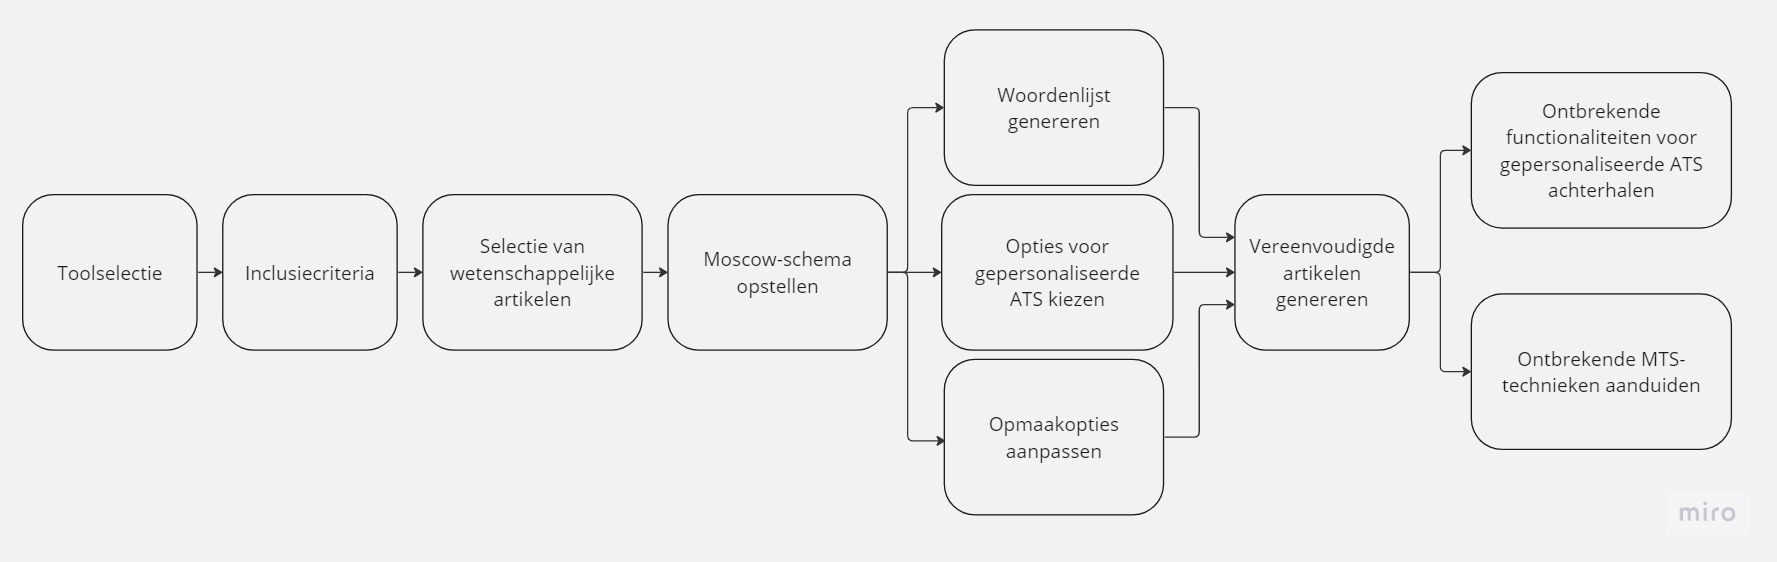
\includegraphics[width=\linewidth]{img/flowchart-requirementsanalyse.jpg}
	\caption{Het benodigde stappenplan bij de requirementanalyse.}
	\label{img:flowchart-requirementsanalyse}
\end{figure}

% TOOLSELECTIE 
Allereerst start het onderzoek met een toolselectie. Zoals aangewezen in sectie \ref{sec:beschikbare-tools-en-taalmodellen}, leent de overheid vijf softwarepakketten uit aan middelbare scholen. Echter neemt de requirementsanalyse drie van deze vijf in de analyse op, want hun functionaliteiten zijn passend voor deze doelgroep. De overige twee zijn minder aanwezig in het onderwijs. Daarnaast toont een zoekopdracht aan dat deze tools geen LS toepassen. Buiten deze erkende softwarepakketten, kunnen online beschikbare tools ook scholieren met dyslexie ondersteunen bij het begrijpend lezen van wetenschappelijke artikelen met ATS, zoals bewezen in \textcite{Bingel2018}. Daarom betrekt de requirementsanalyse enkel tools met onderschreven ATS-functionaliteiten en laat daarmee pure samenvattingstools erbuiten. Tabel \ref{table:shortlist-tools} toont een overzicht van de te experimenteren tools.

\begin{center}
	\begin{table}[H]
		\begin{tabular}{ | m{6cm} | m{6cm} | } 
			\hline
			\textbf{Erkende software} & \textbf{Online beschikbare tools} \\
			\hline
			Sprintplus (E1) & Simplish (O1) \\
			Kurzweil3000 (E2) & SciSpace (O2) \\ 
			AlineaSuite (E3) & Rewordify (O3) \\
			& ChatGPT (O4) \\
			& Bing Chat (O5) \\
			\hline
		\end{tabular}
		\caption{Shortlist van uit te testen tools en toepassingen voor tekstvereenvoudiging.}
		\label{table:shortlist-tools}	
	\end{table}
\end{center}

% Inclusiecritera
Vervolgens bouwt het onderzoek een lijst op van toetsingscriteria. Zo dienen de MTS-technieken uit tabel \ref{table:scientific-paper-struggles} en tabel \ref{table:manual-simplification} als bouwstenen voor het opstellen van de toetsingscriteria. Tabel \ref{table:criteria-requirementsanalysis} geeft een opsomming van de MTS-technieken waaraan tools moeten voldoen. Daarnaast dient dit schema als een inschatting van de functionaliteiten van deze tools.

\begin{center}
	\begin{table}[H]
		\begin{tabular}{ | m{4cm} | m{11cm} | } 
			\hline
			\textbf{MTS-techniek} & \textbf{Functionaliteit} \\
			\hline
			LS & Gepersonaliseerde LS, ofwel woordenschat dat niet te hooggegrepen is. \\
            & Gekende woordenschat mag blijven. \\
			& Woorden met minder lettergrepen gebruiken \\
			& Extra uitleg schrijven bij zinnen \\
			& Paragrafen herschrijven zodat ze eerst uitleg geven op een high-level niveau, vervolgens lagen van complexiteit toevoegen om de lezer te begeleiden \\
			& Woordenlijst aanmaken \\
			& Idiomen vervangen door eenvoudigere synoniemen \\
			\hline
			SS & Zinnen inkorten \\
			& Verwijswoorden aanpassen \\
			& Voorzetseluitdrukkingen aanpassen \\
			& Samengestelde werkwoorden aanpassen \\
			& Actieve stem toepassen \\
			& Enkel regelmatige werkwoorden gebruiken \\
			\hline
			SA & Achtergrondkleur aanpassen \\
			& Woord- en karakterspatiëring \\
			& Consistente lay-out \\
			& Duidelijk zichtbare koppenstructuur \\
			& Huidige positie benadrukken \\
			& Waarschuwingen geven omtrent formulieren en sessies \\
			& Inhoud visueel groeperen \\
			& Tekst herschrijven als tabel \\
			& Tekst herschrijven als opsomming \\
			\hline
		\end{tabular}
		\caption{Richtlijnen waarop het onderzoek de toepassingen aftoetst in de requirementsanalyse.}
		\label{table:criteria-requirementsanalysis}	
	\end{table}
\end{center}

Als realistisch testmateriaal maken de experimenten gebruik van twee gepubliceerde wetenschappelijke artikelen. Zo kunnen deze artikelen relevant zijn voor leerkrachten om aan scholieren in de derde graad van het middelbaar onderwijs te geven als leesvoer. Beide artikelen volgen de kenmerken van een wetenschappelijk artikel, zoals beschreven in tabel \ref{table:scientific-paper-struggles}. Daarnaast gebruiken ze vakjargon en wetenschappelijke concepten in een compact formaat. Tabel \ref{table:referentieteksten-bronvermelding} geeft een overzicht van de twee artikelen en een bijhorende bronvermelding.

\begin{center}
	\begin{table}[H]
		\begin{tabular}{ | m{10cm} | m{5cm} | } 
			\hline
			\textbf{Titel} & \textbf{Bronvermelding} \\
			\hline
			De controle op het gebruik van algoritmische surveillance- onder druk? Een exploratie door de lens van de relationele ethiek & \autocite{VanBrakel2022} \\
			\hline
			Nederland versus België: verschillen in economische dynamiek en beleid. & \autocite{Sleuwaegen2022} \\
			\hline
		\end{tabular}
		\caption{Bronvermeldingen voor de twee wetenschappelijke artikelen.}
		\label{table:referentieteksten-bronvermelding}
	\end{table}
\end{center}

% 4. 
Om een overzicht van de functionaliteiten volgens prioriteit te verkrijgen, bouwt het onderzoek een moscow-schema op vanuit de opgestelde richtlijnen. Zo komen belangrijke functionaliteiten, die nodig zijn om gepersonaliseerde tekstvereenvoudiging met ATS mogelijk te maken, in de categorie \textit{must-haves} terecht. Daarnaast omvatten \textit{should-haves} alle functionaliteiten die niet bijdragen tot gepersonaliseerde ATS, maar wel een meerwaarde biedt in dergelijke toepassingen. Vervolgens bestaan de \textit{could-haves} uit alle functionaliteiten die huidige toepassingen kunnen doen, maar weinig bijdragen tot gepersonaliseerde ATS. Irrelevante functionaliteiten binnen de scope van een prototype of niet toepasselijk voor de doelgroep plaatst het onderzoek als \textit{wont-have}.

\begin{center}
	\begin{table}[H]
		\begin{tabular}{ | m{2cm} | m{13cm} | } 
			\hline
			\textbf{MoSCoW-methode} & \textbf{Functionaliteit} \\
			\hline
			Must-have & Gepersonaliseerde LS, ofwel woordenschat dat niet te hooggegrepen is. Gekende woordenschat mag blijven. \\
			& Woorden met minder lettergrepen gebruiken. \\
			& Woordenlijst aanmaken na handmatige CWI. \\
			& Wetenschappelijke artikelen in PDF-vorm opladen. \\
			& SA-technieken toepassen op de oorspronkelijke tekst. \\
			& Personaliseerbare opmaakopties, waaronder lettertype -en grootte aanpassen, tekstformaat aanpassen, achtergrondkleur aanpassen. \\
			& Duidelijk zichtbare koppenstructuur. \\
			& Tekst herschrijven als opsomming. \\
			\hline
			Should-have & Tekstanalyse \\
			& Extra (in-line) uitleg schrijven bij moeilijke woordenschat. \\
			& Personaliseerbare PDF- of Word-document lay-out. \\
			& Uitvoer als pdf of docx-bestand teruggeven. Het onderzoek gebruikt geen PrintToPDF. \\
			& Wetenschappelijke artikelen in PDF-vorm opladen met OCR. \\
			& Tekstanalyse voor en na de vereenvoudiging aanbieden. \\
			\hline
			Could-have & Huidige positie benadrukken.\\
			& Woordenschat genereren na automatische CWI. \\
			& Waarschuwingen geven omtrent formulieren en sessies. \\
			& Enkel regelmatige werkwoorden gebruiken. \\
			& Extraherende samenvatting \\
			& Abstraherende samenvatting \\
			& Tekst herschrijven in tabelvorm \\
			\hline
			Wont-have & Mobiele versie of \textit{responsive design}. \\
			& Audio-uitvoer \\
			& Integratie met externe toepassingen. Het onderzoek gebruikt Grammarly als voorbeeld voor deze test. \\
			\hline
		\end{tabular}
		\caption{Het moscow-schema voor de requirementsanalyse.}
		\label{img:moscow-table}
	\end{table}
\end{center}

Vervolgens komen experimenten op functionaliteiten voor gepersonaliseerde ATS op wetenschappelijke artikelen aan bod. Allereerst moeten eindgebruikers wetenschappelijke artikelen kunnen opladen. Indien het onderzoek een wetenschappelijk artikel als pdf kan opladen, dan extraheert het de tekstinhoud van het wetenschappelijk artikel. Vervolgens krijgt de toepassing deze tekst als invoer. Zo krijgen de chatbots eerst de prompt, gevolgd door een stuk van het wetenschappelijk artikel. Met zes verschillende prompts kan het onderzoek de LS, SS en SA-functionaliteiten van een promptgebaseerde toepassing achterhalen. Tabel \ref{table:tested-prompts-requirementsanalysis} vermeldt de toegepaste prompts. Toepassingen krijgen eerst een link van het wetenschappelijk artikel. Als de toepassing hier niet over beschikt, dan krijgt de chatbot de tekstinhoud van het wetenschappelijk artikel in \textit{plain-text} mee. 

\begin{center}
	\begin{table}[H]
		\begin{tabular}{ | m{2cm} | m{14cm} | } 
			\hline
			\textbf{Naam} & \textbf{Prompt} \\
			\hline
			P1 & Vereenvoudig deze tekst. \\
			\hline
			P2 & Vereenvoudig deze tekst voor studenten (16-18 jaar) door moeilijke woorden te vervangen, vakjargon te schrappen, woorden langer dan 18 letters te vervangen, acroniemen voluit te schrijven, een woord slechts eenmaal door een synoniem te vervangen, korte uitleg te geven wanneer dat nodig is, en percentages te vervangen. \\
			\hline
			P3 & Vereenvoudig een tekst door deze op te delen in kortere zinnen van maximaal tien woorden. Verander voornaamwoorden als 'zij', 'hun' of 'hij' in namen. Vervang complexe zinsconstructies en voorzetselzinnen door eenvoudiger alternatieven, maar laat ze ongewijzigd als er geen eenvoudiger optie beschikbaar is. \\
			\hline
			P4 & Schrijf de tekst als opsomming. \\
			\hline
			P5 & Schrijf de tekst in tabelformaat. \\
			\hline
			P6 & Genereer op basis van deze tekst een woorden- en synoniemenlijst. \\
			\hline
		\end{tabular}
		\caption{De toegepaste GPT-3-prompts in de requirementsanalyse.}
		\label{table:tested-prompts-requirementsanalysis}
	\end{table}
\end{center}

Daarna voert het onderzoek experimenten uit rond gepersonaliseerde opmaakopties. Kurzweil, SprintPlus en AlineaSuite bieden opmaakopties aan in het instellingenscherm. Zo kunnen eindgebruikers het lettertype, -kleur, -grootte en de achtergrondkleur van de tekst aanpassen naar keuze. Als een toepassing niet over opmaakopties beschikt, stopt het experiment rond opmaakopties voor die toepassing. Tot slot test het onderzoek de mogelijkheden om het formaat van teksten aan te passen met structurele aanpassingen. Zo vragen P4 en P5 specifiek naar een structurele aanpassing, terwijl P1, P2 en P3 minstens een doorlopende tekst als resultaat verwachten. Andere beschikbare tools missen checkboxen of keuzelijsten om deze keuze aan te reiken, waardoor het testen van deze functionaliteit niet mogelijk is.

\section{Vergelijking van taalmodellen}
\label{sec:vergelijkende-studie}

Om wetenschappelijke artikelen met gepersonaliseerde ATS te vereenvoudigen, moet een dergelijk toepassing gebruikmaken van een geschikt taalmodel. Zo moet Pentimentor vereenvoudigde versies van wetenschappelijke artikelen kunnen geven, specifiek volgens de noden van scholieren met dyslexie in de derde graad van het middelbaar onderwijs. Om de uitvoer van het prototype nauwkeurig af te stemmen, moet het onderzoek een antwoord geven op de volgende vraag.

\begin{itemize}
	\item Welk taalmodel kunnen ontwikkelaars inzetten voor tekstvereenvoudiging met ATS van wetenschappelijke artikelen voor scholieren met dyslexie in de derde graad van het middelbaar onderwijs, met dezelfde of gelijkaardige kwaliteiten als gepersonaliseerde tekstvereenvoudiging met MTS?
\end{itemize}

Zoals in de literatuurstudie aangegeven, beschikken ontwikkelaars over onvoldoende gespecialiseerde taalmodellen om wetenschappelijke artikelen te vereenvoudigen. Daarom vergelijkt deze onderzoeksfase alle taalmodellen uit tabel \ref{table:vergelijkende-studie-taalmodellen}. 

\begin{center}
	\begin{table}[H]
		\begin{tabular}{ | m{4cm} | m{11cm} | } 
			\hline
			\textbf{Verwijzing} & \textbf{Taalmodel} \\
			\hline
			T1 & Haining Scientific Abstract Simplification \\
			\hline
			T2 & BART-based Scientific Lay Summarizer \\
			\hline
			T3 & Keep It Simple\\
			\hline
			T4 & GPT-3 \\
			\hline
		\end{tabular}
		\caption{Gebruikte taalmodellen in de vergelijkende studie}
		\label{table:vergelijkende-studie-taalmodellen}
	\end{table}
\end{center}

Deze onderzoeksfase bestaat uit vijf deelfasen, weergegeven op figuur \ref{img:flowchart-vergelijkende-studie-metrics}. Het staat vooral stil bij de vergelijking van leesmetrieken van de oorspronkelijke wetenschappelijke artikelen, MTS-referentieteksten en ATS-teksten. Met een \textit{mixed-methods} onderzoek kan deze onderzoeksfase taalmodellen beoordelen op machinaal en menselijk niveau. Alle scripts kan de lezer terugvinden op de GitHub-repository\footnote{https://github.com/Dyashen/pentimentor/tree/main/bachelorproef/scripts}. Het onderzoek hergebruikt dezelfde wetenschappelijke artikelen als in de requirementsanalyse, namelijk die in tabel \ref{table:referentieteksten-bronvermelding}. Om realistisch referentiemateriaal te verkrijgen, schrijven twee leerkrachten (MTSL) en twee leerlingen zonder dyslexie (MTSL2) zelf een vereenvoudiging van de twee wetenschappelijke artikelen met MTS. Deze vier personen baseren zich op vooraf meegekregen richtlijnen, toegelicht in bijlage \ref{ch:referentietekst}. 

\begin{figure}
	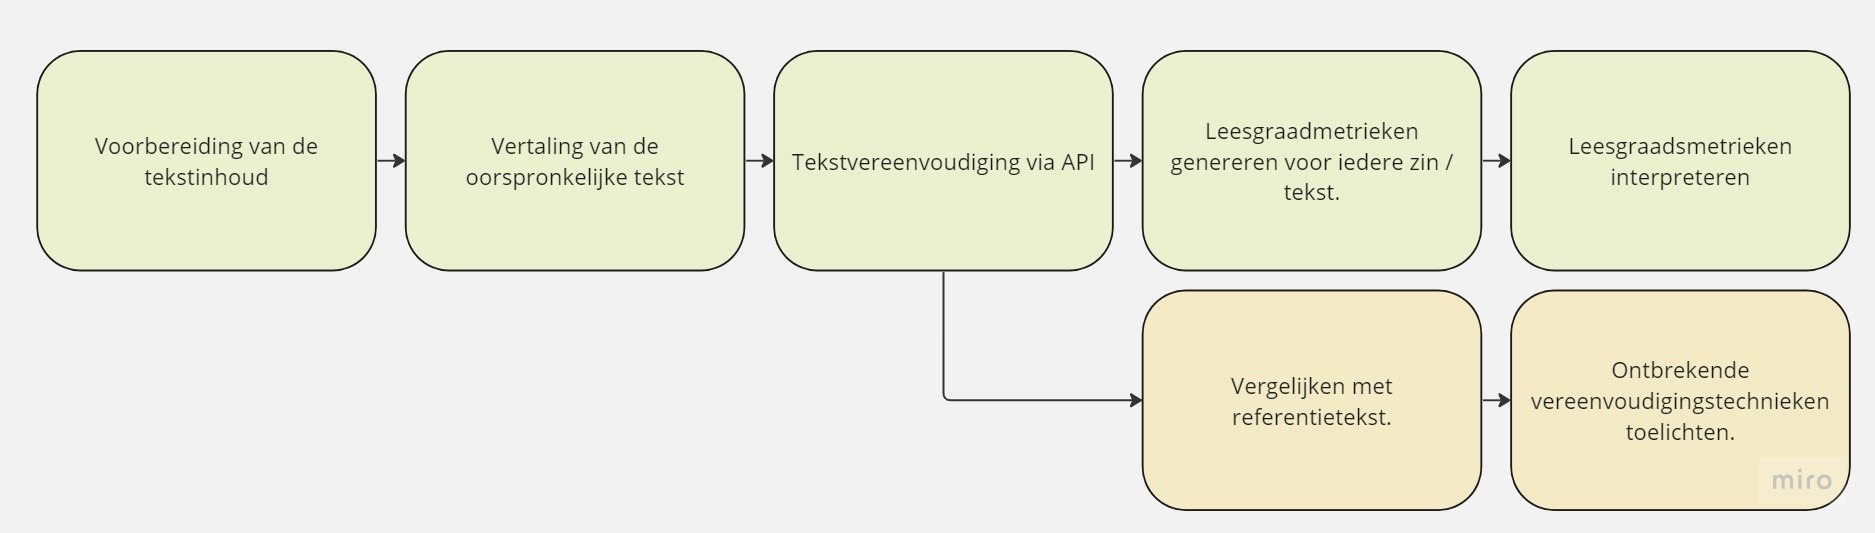
\includegraphics[width=\linewidth]{img/flowchart-vergelijkende-studie.jpg}
	\caption{Het gevolgde stappenplan voor de vergelijking van taalmodellen.}
	\label{img:flowchart-vergelijkende-studie-metrics}
\end{figure}

Allereerst haalt het script de inhoud van de map op met wetenschappelijke artikelen om deze vervolgens in een tekstbestand te plaatsen, zoals weergegeven in codeblok \ref{code:verg-studie-phase-1}. Hier schrijft het script tekstinhoud van het wetenschappelijk artikel over naar een nieuw tekstbestand.

\begin{lstlisting}[language=Python, caption={Script voor de eerste fase van de vergelijkende studie.}, label={code:verg-studie-phase-1}]
def add_newline_after_dot(input_file, output_file):
	with open(input_file, 'r', encoding='utf-8') as file:
		text = file.read()
		text = re.sub(r'\d', '', text)
		modified_text = text.replace('.', '.\n')
		with open(output_file, 'w', encoding='utf-8') as file:
			file.write(modified_text)
		
		folder_path = 'scripts\pdf'
		original_scientific_papers = [f for f in os.listdir(folder_path)]
		
		for paper in original_scientific_papers:
			input_file =  folder_path + '/' + paper
			output_file = folder_path + '/' + 'RE_' + paper
			add_newline_after_dot(input_file, output_file)
\end{lstlisting} 

Vervolgens vertaalt het tweede script alle zinnen naar het Engels. Eerst doorloopt het alle zinnen binnen het wetenschappelijk artikel. Daarna vertaalt het de tekstinhoud met de \textit{deep translator} python-bibliotheek. Als resultaat ontstaat er een csv-bestand met twee kolommen: alle Nederlandstalige en alle Engelstalige zinnen van één wetenschappelijk artikel. Als separator gebruikt het csv-bestand een \textit{pipe}-symbool en zo houdt het rekening met punten en komma's in zinnen.

\begin{center}
	\begin{lstlisting}[language=Python, caption={Script voor de tweede fase van de vergelijkende studie.}, label={code:verg-studie-phase-2}]
def translate_dutch_to_english(dutch_text_file):
	with open(dutch_text_file, 'r', encoding='utf-8') as file:
		dutch_sentences = file.readlines()
		dutch_sentences = [sentence.strip() for sentence in dutch_sentences]
				
		english_sentences = []
		for sentence in dutch_sentences:
			translated = GoogleTranslator(source='nl', target='en').translate(sentence)
			english_sentences.append(translated)
			df = pd.DataFrame({'Dutch': dutch_sentences, 'English': english_sentences})
			df.to_csv(str(dutch_text_file).split('.')[0] + '.csv', index=False)
				
				
		folder_path = 'scripts/pdf/'
		original_scientific_papers = [f for f in os.listdir(folder_path)]
				
		for paper in original_scientific_papers:
			if paper.startswith('RE_') and paper.endswith('.txt'):
				print(f'STARTING {paper}')
				dutch_text_file = folder_path + paper
				translate_dutch_to_english(dutch_text_file)
		\end{lstlisting}
\end{center}

In een derde fase moet het script API-calls voor iedere zin of paragraaf versturen naar ieder taalmodel. Eerst slaat het script een \textit{dictionary} op van taalmodellen om de inhoud van de wetenschappelijke artikelen te vereenvoudigen, zoals weergegeven in listing \ref{code:verg-studie-phase-3}. Daarna vindt tokenisatie plaats, waarvoor het script Spacy \textit{sentence tokenisation} en verwante \textit{embedding models} gebruikt. Deze modellen staan in tabel \ref{table:wordembeddings-spacy}. Na de tokenisatie stuurt het script API-calls naar de hosts van de taalmodellen. Het verzoek naar de \textit{HuggingFace} (HF) API bestaat uit de parameters weergegeven in tabel \ref{table:huggingface-requests-parameters}. Alle HF-taalmodellen vereisen een laadfase. Daarom bevat de \textit{API-call} een extra parameter, namelijk \textit{wait\_for\_model}. Verder past dit script geen extra parameters van de taalmodellen aan. 

\begin{center}
	\begin{table}[H]
		\begin{tabular}{ | m{6cm} | m{8cm} | } 
			\hline
			\textbf{Naam parameter} & \textbf{Waarde} \\
			\hline
			Inputs & De oorspronkelijke zin. Enkel bij T1 komt 'simplify:' voor deze zin. \\
			\hline
			Max length & De lengte van de oorspronkelijke zin + 10 tokens. \\
			\hline
			Wait for model & Altijd ingesteld op \textit{True}. \\
			\hline
		\end{tabular}
		\caption{Meegegeven parameters bij HF-requests}
		\label{table:huggingface-requests-parameters}
	\end{table}
\end{center}

Zoals aangehaald door \textcite{Gooding2022} kunnen promptgebaseerde testen verschillende resultaten leveren, afhankelijk van de gegeven input. Daarom gebruikt het script drie verschillende prompts, gebaseerd op de MTS-technieken beschreven in tabel \ref{table:manual-simplification}. Tabel \ref{table:tested-prompts} visualiseert de gebruikte prompts voor de testen met het GPT-3 model. 

\begin{center}
	\begin{table}[H]
		\begin{tabular}{ | m{2cm} | m{13cm} | } 
			\hline
			\textbf{Naam} & \textbf{Prompt} \\
			\hline
			P1 & Vereenvoudig deze tekst \\
			\hline
			P2 & Vereenvoudig deze tekst voor studenten (16-18 jaar) door moeilijke woorden te vervangen, vakjargon te schrappen, woorden langer dan 18 letters te vervangen, acroniemen voluit te schrijven, een woord slechts eenmaal door een synoniem te vervangen, korte uitleg te geven wanneer dat nodig is, en percentages te vervangen. \\
			\hline
			P3 & Vereenvoudig een tekst door deze op te delen in kortere zinnen van maximaal tien woorden. Verander voornaamwoorden als 'zij', 'hun' of 'hij' in namen. Vervang complexe zinsconstructies en voorzetselzinnen door eenvoudiger alternatieven, maar laat ze ongewijzigd als er geen eenvoudiger optie beschikbaar is. \\
			\hline
		\end{tabular}
		\caption{De GPT-3-prompts die in de vergelijkende studie aan bod komen.}
		\label{table:tested-prompts}
	\end{table}
\end{center}

Zowel T1 als T4 gebruiken een \textit{nul-temperature} en een \textit{top-p} waarde van 90\% om vertrouwde antwoorden te krijgen. Daarnaast dient de top-p om een hoge woordfrequentie te verkrijgen, zoals aangegeven in tabel \ref{table:gpt-3-parameters}. Bij T1 zijn deze twee parameters ingebakken in de functie. Nadien verwerken de taalmodellen iedere zin uit de tekst. Tot slot geeft de HF of GPT-3 API een resultaat in JSON-formaat, bevattende de vereenvoudigde versie van de opgegeven zin. T1, T2 en T3 vereenvoudigen de Engelstalige zinnen, in tegenstelling tot T4 en verwante prompts die de Nederlandstalige zinnen vereenvoudigen. Om een \textit{request failure} door een te lange input te voorkomen, breekt het script de volledige input op per 1000 tokens.

\begin{center}
	\begin{table}[H]
		\begin{tabular}{ | m{7cm} | m{7cm} | } 
			\hline
			\textbf{Taal} & \textbf{Embeddingsmodel} \\
			\hline
			Nederlands & NL Core News Medium \\ 
			\hline
			Engels & EN Core Web Medium \\
			\hline
		\end{tabular}
		\caption{Gebruikte SpaCy word-embeddings}
		\label{table:wordembeddings-spacy}
	\end{table}
\end{center}

\begin{center}
	\begin{lstlisting}[language=Python, caption={Script voor de derde fase van de vergelijkende studie}, label={code:verg-studie-phase-3}]
 def scientific_simplify(self, text, lm_key):
    try:
        API_URL = huggingfacemodels.get(lm_key)
        translated = GoogleTranslator(source='auto', target='en').translate(str(text))
    
        if lm_key == 'T1':
            result = self.query({"inputs": str('simplify: ' + str(translated)),"parameters": {"max_length": len(sentence)+10},"options":{"wait_for_model":True}}, API_URL)
        else:
            result  = self.query({"inputs": str(translated),"parameters": {"max_length": len(sentence)+10},"options":{"wait_for_model":True}}, API_URL)
    
        if 'generated_text' in result[0]:
            translated = GoogleTranslator(source='auto', target='nl').translate(str(result[0]['generated_text']))
            return translated
        elif 'summary_text' in result[0]:
            translated = GoogleTranslator(source='auto', target='nl').translate(str(result[0]['summary_text']))
            return translated
        else:
            return None
        except:
            return text		
            
hf = HuggingFaceModels(os.getenv('huggingface-api-key'))
original_scientific_papers = [f for f in os.listdir(folder_path)]
for paper in original_scientific_papers:
    sentence_tokens = process_file(paper) 
        for sentence in sentence_tokens:
            for model in huggingfacemodels.keys():
                filename = "SIMPLIFIED_"+model+'_'+paper
                with open(filename, 'a', encoding='utf-8') as f:
                    output = hf.scientific_simplify(str(sentence), model)
                    f.write(str(output)) 
	\end{lstlisting}
\end{center}

Vervolgens berekent het script leesmetrieken met de \textit{readability} python-bibliotheek. Leesmetrieken dienen als objectieve maatstaf bij deze vergelijkende studie, zoals aangegeven door \textcite{Nenkova2004}. 

\begin{itemize}
	\item De vergelijkende studie neemt de Flesch-Reading-Ease (FRE) en Gunning FOG (FOG) scores op, want deze scores kunnen de moeilijkheidsgraad van een zin of tekst machinaal meten.
	\item Het aantal complexe en lange woorden kan wijzen op de gebruikte \textit{substitution generation} van het taalmodel. De \textit{Dale-Chall Index} bepaalt de complexiteit van een woord in deze library. Ten slotte tellen alle woorden met meer dan vier lettergrepen mee als een lang woord volgens de \textit{readability}-library.
	\item Het aantal hulpwerkwoorden en vervoegingen van 'zijn' kan aanduiden op mogelijke passieve stem, wat het onderzoek van \textcite{Ruelas2020} als 'hinderende' zinsyntax vernoemt.
\end{itemize}

Dit script resulteert in een \textit{Pandas-dataframe} met alle leesbaarheidsmetrieken uit de \textit{readability}-library. Uiteindelijk slaat het script de \textit{Pandas-dataframe} op als csv-bestand. Listing \ref{code:verg-studie-phase-4} omvat de code voor fase 4. Hierin berekent het script de leesmetrieken voor iedere zin. Allereerst laadt het script twee embeddingsmodellen in, weergegeven in tabel \ref{table:wordembeddings-spacy}. Daarna bouwt het lege dataframes op om de meetresultaten te kunnen opslaan. Vervolgens itereert het python-script door alle tekstbestanden om deze tekst in te lezen. Voor elke zin probeert het script leesmetrieken te verkrijgen met de \textit{readability.getmeasures} functie. Hierbij specifieert het script welke taal de readability-library moet gebruiken. Als het script alle meetwaarden succesvol kan verkrijgen, dan maakt het script een nieuwe rij met machinaal berekende leesmetrieken. Tot slot voegt het alle rijen toe aan de DataFrame. Het script verwerpt de zinnen voor het specifieke artikel waarbij het geen leesmetrieken kan berekenen.

\begin{center}
	\begin{lstlisting}[language=Python, caption={Script voor de vierde fase van de vergelijkende studie}, label={code:verg-studie-phase-4}]	
		simplified_folder = 'scripts/vereenvoudigde_artikelen'
		original_folder = 'scripts/pdf'
		
		scientific_papers = [original_folder + "/" + f for f in os.listdir(original_folder)] + [simplified_folder + "/" + f for f in os.listdir(simplified_folder)]
		
		languages = {
			'nl':'nl_core_news_md',
			'en':'en_core_web_md'
		}
		
		df = pd.DataFrame()
		
		for paper in scientific_papers:
		with open(paper, 'r', encoding='utf-8') as file:
			text = file.read()
			nlp = spacy.load(languages.get('nl'))
			doc = nlp(text)
		
		for sent in doc.sents:
			try:
				metrics = readability.getmeasures(sent.text, lang='nl')
				row = {
					'Paper': paper.split('/')[2].split('.')[0],
					'Sentence': sent.text,
					'FRE': metrics['readability grades']['FleschReadingEase'],
					'FOG': metrics['readability grades']['GunningFogIndex'],
				}
		
		for key, value in metrics['sentence info'].items():
			row[key] = value
		
		for key, value in metrics['word usage'].items():
			row[key] = value
		
		for key, value in metrics['sentence beginnings'].items():
			row[key] = value
			
		df = df.append(row, ignore_index=True)
		except Exception as e:
			print(e)
		
		df.to_csv('result.csv', index=False)
	\end{lstlisting}
\end{center}

In de laatste fase visualiseert het onderzoek de verkregen resultaten. Hierbij gebruikt het \textit{Jupyter-notebooks} en \textit{Matplotlib} om de verkregen resultaten voor te stellen. Allereerst gebruikt de \textit{Jupyter-notebook} een kleinere dataframe met enkel de data van A1. Daarna groepeert het script de data op basis van modellen. Het aantal woorden per zin fungeert als geaggregeerd veld. Met Matplotlib kan het script vervolgens een eenvoudige boxplot genereren. De notebook herhaalt dit proces voor beide artikelen en voor alle leesmetrieken vermeldt in tabel \ref{table:verg-studie-metrieken}. Zo illlustreert \textit{listing} \ref{code:generation-boxplot} hoe het script boxplots genereert. Deze visualiseren het woordgebruik van de verschillende taalmodellen bij A1. Alle code om grafieken te genereren kan de lezer op de GitHub-repository\footnote{https://github.com/dylancluyse/bachelorproef-nlp-tekstvereenvoudiging/blob main/scripts/PHASE\_5.ipynb} terugvinden. 

\begin{lstlisting}[language=Python, caption={Code om een boxplot voor het aantal woorden per zin te genereren.}, label={code:generation-boxplot}]	
artikel_1 = df[(df['paper'] == 'Artikel 1 AI') & (df['FRE'] > 0)]
data = artikel_1.groupby('model')['words_per_sentence']
data_list = [group[1].tolist() for group in data]
plt.figure(figsize=(20,10))
plt.boxplot(data_list)
plt.xticks(range(1, len(data_list) + 1), data.groups.keys())
plt.title('Woorden per zin per model')
plt.xlabel('Model')
plt.ylabel('Woorden per zin')
plt.savefig('boxplot-avg-a1.png')
\end{lstlisting}

Verder toont tabel \ref{table:verg-studie-metrieken} alle leesmetrieken, samen met de toegepaste visualisatietechniek. De boxplots dienen om de spreiding van de leesmetrieken te tonen. Zo kan het onderzoek achterhalen hoe gespreid de gebruikte woordenschat is op het vlak van de leesmetrieken FRE en FOG. De spreiding bij het aantal woorden per zinnen geeft het onderzoek ook weer als een boxplot. Zo kan het onderzoek de regelmaat van korte zinnen achterhalen uit een tekst. De \textit{violinplots} dienen om de verdeling van moeilijke of lange woorden weer te geven. Tot slot maakt het onderzoek gebruik van een staafdiagram om het aantal hulpwerkwoorden of aantal zinnen met een vervoeging van het werkwoord 'zijn' te visualiseren.

\begin{center}
	\begin{table}[H]
		\begin{tabular}{ | m{8cm} | m{7cm} | } 
			\hline
			\textbf{Leesmetriek} & \textbf{Visualisatietechniek }\\
			\hline
			FOG & Boxplot \\
			\hline
			FRE & Boxplot \\
			\hline
			Aantal woorden per zinnen & Boxplot \\
			\hline
			Aantal complexe woorden per zin volgens Dale Chall index & Violinplot \\
			\hline
			Aantal lange woorden per zin & Violinplot \\
			\hline
			Aantal gebruikte hulpwerkwoorden & Staafdiagram \\
			\hline
			Aantal zinnen met een vervoeging van het werkwoord 'zijn' & Staafdiagram \\
			\hline
		\end{tabular}
		\caption{Visualisatietechnieken voor de machinale metrieken bij de vergelijking van de vereenvoudigde teksten met de oorspronkelijke tekst en de referentieteksten.}
		\label{table:verg-studie-metrieken}
	\end{table}
\end{center}

Tenslotte komen de resultaten van de menselijke beoordeling aan bod. Deze fase van de vergelijkende studie staat stil bij aspecten die de leesmetrieken niet kunnen meten, waaronder de normen vermeld in tabel \ref{table:criteria-vergelijkende-studie-human-obv}. De referentietekst dient hier als hulpmiddel om de referentietekst, ofwel het verwachte resultaat, te vergelijken met de vereenvoudigde tekst door een taalmodel. 

\begin{table}[H]
	\begin{tabular}{| m{10cm} | m{4.5cm} |}
		\hline
		\textbf{Metriek} & \textbf{Vereenvoudigings- techniek} \\ \hline
		Acroniemen behouden & LS 	\\ \hline
		Inschatting van de doelgroep & LS	\\ \hline
		Behoud van kern- en bijzaken & LS \\ \hline
		Schrijven in tabelvorm of als opsomming & SA \\ \hline
		Passieve zinconstructies herschrijven naar actieve zinconstructies & SS \\ \hline
		Bronvermelding behouden &  SA \\ \hline
		Citeren en parafraseren & SS en SA. \\ \hline
	\end{tabular}
	\caption{Criteria voor menselijke observatie bij de vergelijkende studie.}
	\label{table:criteria-vergelijkende-studie-human-obv}
\end{table}

\section{Prototype voor tekstvereenvoudiging}

Met de gevonden vereisten voor een taalmodel uit het moscow-schema en de geschikte taalmodellen voor gepersonaliseerde ATS kan het onderzoek een volgende stap zetten om de onderzoeksvraag te beantwoorden. De volgende sectie omschrijft de ontwikkeling van Pentimentor, namelijk een prototype voor gepersonaliseerde ATS voor scholieren met dyslexie in de derde graad van het middelbaar onderwijs. Deze ontwikkeling kan ontwikkelaars helpen als rode draad bij het maken van dergelijke toepassingen. Zo beantwoordt de ontwikkeling van \textit{Pentimentor} volgende deelvraag: 

\begin{itemize}
	\item Hoe kunnen ontwikkelaars een intuïtieve en lokale webtoepassing ontwikkelen die zowel scholieren met dyslexie als leerkrachten kan helpen bij het vereenvoudigen van wetenschappelijke artikelen met behoud van semantiek, jargon en zinsstructuren?
\end{itemize}

Voor de ontwikkeling van het prototype volgt het onderzoek figuur \ref{img:general-overview-prototype}. Deze flowchart toont zes algemene fasen. Zo start het onderzoek met een voorbereidende fase waarin het onderzoek de nodige technieken en taalmodellen opsomt. Vervolgens ontwikkelt het de backend en frontend. Daarna ontwikkelt het twee algemene componenten: een leraren -en scholierencomponent. Hierna moet het onderzoek stilstaan bij de opzet van Pentimentor. 

\medspace

Uiteindelijk beoordeelt het onderzoek de \textit{Pentimentor} prototype. Het vergelijkt dit met andere toepassingen volgens het moscow-schema. Zo moet het lerarencomponent wetenschappelijke artikelen kunnen vereenvoudigen, nadat de gebruiker ATS-technieken selecteert. Daarnaast moet het scholierencomponent ondersteuning bieden aan scholieren die de verschillen tussen de originele en vereenvoudigde tekst willen zien. Hier moeten scholieren met dyslexie in \textit{real-time} aanpassingen kunnen maken aan de tekst en ondersteuning krijgen tijdens het begrijpend lezen van een tekst. Tot slot moeten gepersonaliseerde opmaakopties gelijk blijven over alle pagina's heen van Pentimentor.


\begin{sidewaysfigure}
	\begin{figure}[H]
		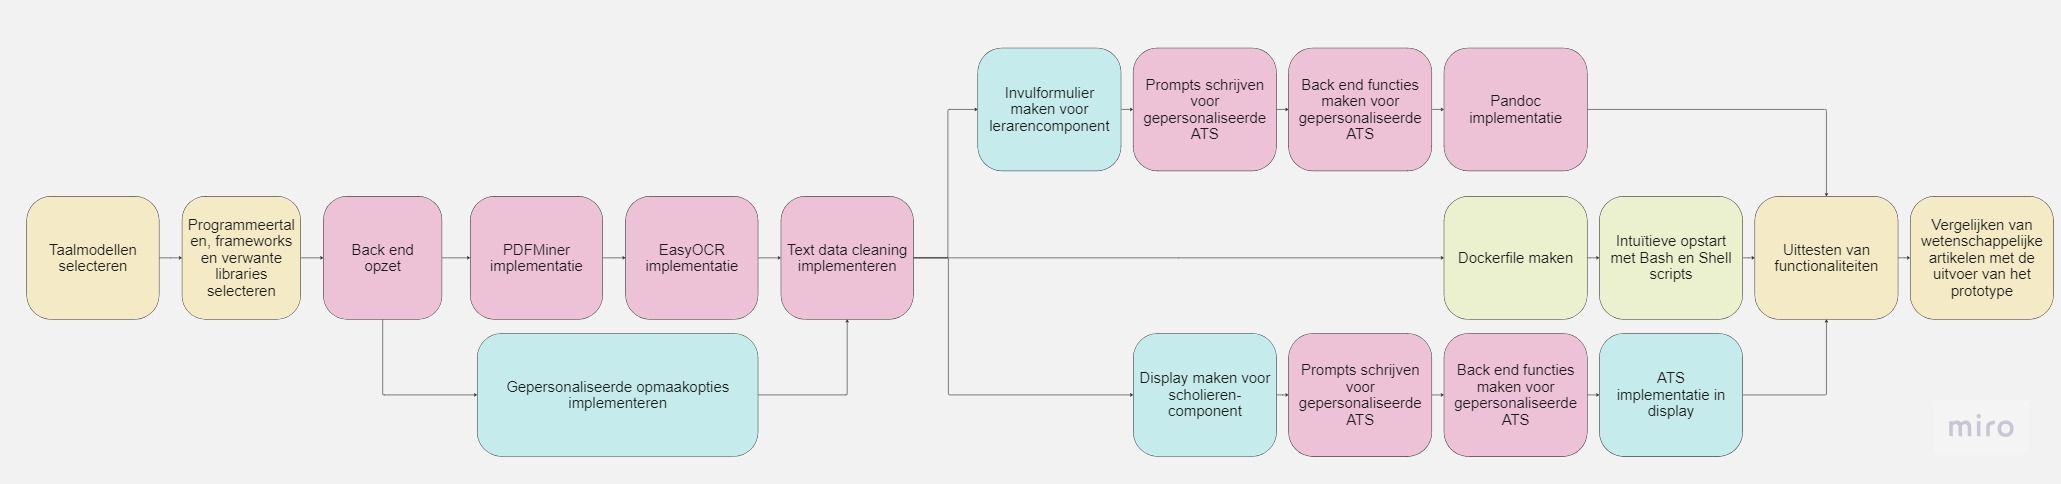
\includegraphics[width=\linewidth]{img/flowchart-general-development.jpg}
		\caption{Algemeen overzicht van de ontwikkeling van het prototype voor ATS van wetenschappelijke artikelen.}
		\label{img:general-overview-prototype}
	\end{figure}
\end{sidewaysfigure}

\subsubsection{Taalmodellen selecteren}

Omdat de keuze van taalmodellen verdere technologiekeuzes kan beïnvloeden, bepaalt het onderzoek eerst één of meerdere taalmodellen voor gepersonaliseerde ATS. Zo wijst de vorige onderzoeksfase uit dat GPT-3 een geschikt taalmodel is voor gepersonaliseerde ATS. Voor een abstraherende samenvatting kan \textit{Pentimentor} één van drie taalmodellen uit de vorige onderzoeksfase gebruiken.

\subsubsection{Programmeertalen, frameworks en verwante libraries selecteren}

Voor een snelle en gratis ontwikkeling gebruikt \textit{Pentimentor} \textit{open-source} pakketten. Taalmodellen kunnen het aanspreken via \textit{API-calls} met JS of Python. Omdat het systeem de API-sleutel moet opslaan als sessievariabele, gebeuren alle \textit{API-calls} vanuit de backend. Verder vermeldt tabel \ref{table:technologies} alle gebruikte programmeertalen. Tot slot vermeldt tabel \ref{table:python-libraries} alle gebruikte python-libraries.

\begin{center}
	\begin{table}[H]
	\begin{tabular}{ | m{4cm} | m{11cm} | } 
		\hline
		\textbf{Technologie} 	& \textbf{Functionaliteit} \\
		\hline
		Python 					& Dit dient voor de backend die API-calls en PoS-tags verwerkt. \\
		\hline
		JavaScript (JS)			& Dit maakt de toepassing eenduidig door CLI-instructies te vervangen door knoppen. \\
		\hline
		HTML en CSS 			& Dit past het uiterlijk aan, naargelang de gekozen parameters van de eindgebruiker. \\
		\hline
		Jinja 					& Dit geeft alle Python backend data door aan de frontend.  \\
		\hline
		Docker 					& Dit dient om Pentimentor lokaal op te kunnen starten en voorziet een lokale omgeving waarin het systeem alle software installeert. \\
		\hline
		Bash					& Script om de lokale opzet op eenduidige wijze op te starten voor Linux en Mac-systemen. \\
		\hline
		Powershell 				& Script om de lokale opzet op eenduidige wijze op te starten voor Windows-systemen. \\
		\hline
	\end{tabular}
	\caption{Gebruikte programmeertalen in het prototype voor tekstvereenvoudiging.}
	\label{table:technologies}
	\end{table}
\end{center}

\begin{center}
	\begin{table}[H]
	\begin{tabular}{ | m{4cm} | m{11cm} | } 
		\hline
		\textbf{Python-bibliotheek} & \textbf{Functionaliteit} \\
		\hline
		Flask					& Het websiteframework van Pentimentor. Dit framework combineert frontend en backend. \\ 
		\hline
		PDFMiner 				& Tekstinhoud van PDF's extraheren. \\ 
		\hline
		LayoutParser			& Selectief tekstinhoud uit PDF's extraheren. \\
		\hline
		NumPy 					& De \textit{reshape}-functie vereenvoudigt de ontwikkeling om dynamisch paragrafen uit te printen. \\
		\hline		
		Spacy 					& \textit{PoS-tagging} en \textit{token lemmatization}. \\
		\hline
		OpenAI					& GPT-3 API aanspreken. \\
		\hline
	\end{tabular}
	\caption{Gebruikte Python-libraries en hun respectievelijke functie in het prototype.}
	\label{table:python-libraries}
	\end{table}
\end{center}

\subsubsection{Backend opzet}

Nadat het onderzoek taalmodellen, technologieën en frameworks uitkiest, start het met de frontend implementatie. Allereerst voegt het de homepagina toe. Dit dient als portaal voor de componenten. Daarna implementeert het personaliseerbare opmaakopties. Zoals aangeraden door \textcite{Galliussi2020}, moeten ontwikkelaars hiermee rekening houden. Zo gebruikt Pentimentor parameters onderzocht door \textcite{Rello2013a, Rello2013b}. Om deze instellingen aan te bieden, voegt het onderzoek een webpagina toe. Deze HTML-pagina bevat formulieren met aanpasbare parameters. Nadat de gebruiker parameters aanpast, stuurt de pagina een POST-request naar de backend. Het verwerkt dit en slaat de ontvangen dictionary op als sessievariabele, zoals weergegeven in listing \ref{code:back-end-session-personalized}. Tot slot laadt de frontend deze opmaakopties in bij iedere wegpagina. Dit gebeurt met \textit{window onload}, zoals weergegeven in listing \ref{code:window-onload-js}. Zo hoeven eindgebruikers deze parameters niet bij iedere webpagina opnieuw aan te passen.


\begin{lstlisting}[language=python, caption={De backend functie die de aanpassingen uit het formulier opslaat als sessievariabele.}, label={code:back-end-session-personalized}]
PER_SET_SESSION_NAME = 'personalized_settings'

@app.route('/get-settings-user',methods=['POST'])
def return_personal_settings_dict():
	if PER_SET_SESSION_NAME in session:
		return jsonify(session[PER_SET_SESSION_NAME])
	else:
		return jsonify(result='session does not exist')
	
@app.route('/change-settings-user', methods=['POST'])
def change_personal_settings():
	try:
		session[PER_SET_SESSION_NAME] = dict(request.form)
		msg = 'Succesvol aangepast!'
	except Exception as e:
		msg = str(e)
		flash(msg)
	return render_template('settings.html')
\end{lstlisting}

\begin{lstlisting}[language=javascript, caption={De onload-functie die de gepersonaliseerde opmaakopties regelt bij het inladen van een webpagina.}, label={code:window-onload-js}]
window.onload = async function () {
	var url = `http://localhost:5000/get-settings-user`;
	const response = await fetch(url, { method: 'POST' });
	var result = await response.json();
	document.body.style.fontSize        = result.fontSize+'px';
	document.body.style.fontFamily      = result.fontSettings;
	document.body.style.backgroundColor = result.favcolor;
	document.body.style.lineHeight      = result.lineHeight+'cm';
	document.body.style.wordSpacing     = result.wordSpacing+'cm';
	document.body.style.textAlign       = result.textAlign;
}
\end{lstlisting}

Naast personaliseerbare opmaakopties moet \textit{Pentimentor} wetenschappelijke artikelen kunnen inladen en inlezen. Zo kan het met \textit{PDF-extractors} zoals \textit{PDFMiner} tekst uit de PDF extraheren. Niet alle \textit{PDF-extractors} zijn foutbestendig, want zoals opgemerkt in de literatuurstudie kunnen \textit{PDF-extractors} ook tekst verliezen tijdens dit proces. Om dit te voorkomen, biedt het prototype een OCR-optie met \textit{LayoutParser} aan. Beide manieren vereisen functies in de backend en frontend.

\medspace

Aan de frontend voegt het onderzoek checkboxes, file-input en texarea-input tags toe. Uiteindelijk stuurt het formulier een POST-request om alle meegekregen informatie door te sturen naar de backend. Na het ontvangen van de request van de frontend, handelt de Flask backend het bestand verder af zoals aangewezen in listing \ref{code:inlezen-wetenschappelijk-artikel-front-end-back-end}. Nadat de gebruiker het formulier bevestigt, geeft het de binaries van het wetenschappelijk artikel door aan de backend. Die controleert het type invoer en slaat het nadien tijdelijk \textit{in-memory} op. Daarnaast krijgt het de keuze tussen normale of OCR-upload mee als boolean, waarbij \textit{true} gelijk staat aan een afhandeling met LayoutParser.

\begin{lstlisting}[language=Python, caption={Koppeling tussen frontend en backend voor het inlezen van een wetenschappelijk artikel}, label={code:inlezen-wetenschappelijk-artikel-front-end-back-end}]
def setup_scholars_teachers(request):
	settings = request.form
	if 'fullText' in request.form:
		text = request.form['fullText']
		langs = detect_langs(text)
		reader = Reader()
		dict_text = reader.get_full_text_site(text)                
	elif 'pdf' in request.files:
		if 'advanced' not in settings:
			pdf = request.files['pdf']
			pdf_data = BytesIO(pdf.read())
			all_pages = extract_pages(pdf_data,page_numbers=None,maxpages=999)
			langs = detect_langs(str(all_pages))
			reader = Reader()
			full_text = reader.get_full_text_dict(all_pages)
			dict_text = reader.get_full_text_site(full_text)
		else:
			pdf = request.files['pdf']
			pdf_data = pdf.read()
			pages = convert_from_bytes(pdf_data)
			reader = Reader()
			img_text = reader.get_full_text_from_image(pages)
			langs = detect_langs(img_text)
			dict_text = reader.get_full_text_site(img_text)                            
			return dict_text, langs, 'voorbeeldtitel', 'voorbeeldonderwerp'
			
@app.route('/for-scholars', methods=['GET','POST'])
def teaching_tool():
	try:
		dict_text, langs, title, subject = setup_scholars_teachers(request)
		return render_template('for-scholars.html', pdf=dict_text, lang=langs, title=title, subject=subject)
	except Exception as e:
		return render_template('error.html',error=str(e))
	
@app.route('/for-teachers', methods=['GET','POST'])
def analysing_choosing_for_teachers():
	try:
		dict_text, langs, title, subject = setup_scholars_teachers(request)
		return render_template('for-teachers.html', pdf=dict_text, lang=langs, title=title, subject=subject)
	except Exception as e:
		return render_template('error.html',error=str(e))
\end{lstlisting}

\subsubsection{PDFMiner implementatie}

Bij een gewone PDF-extractie gebruikt de Reader-klasse PDFMiner met de functie in listing \ref{code:inlezen-van-pdf}. Het itereert door alle pagina's van een opgeladen wetenschappelijk artikel. Nadien extraheert het alle tekst van een pagina en concateneert het alle opgehaalde tekst van één pagina aan een lege string. Dit proces herhaalt zich tot het geen pagina's meer kan inlezen. Tot slot resulteert dit in een string-object met alle geëxtraheerde tekst uit het wetenschappelijk artikel. Hierna moet de Reader-klasse deze tekst formatteren tot een leesbaar formaat.

\begin{lstlisting}[language=Python, caption={Een PDF inlezen met PDFMiner}, label={code:inlezen-van-pdf}]
	def get_full_text_from_pdf(self, all_pages):
		total = ""
		for page_layout in all_pages:
			for element in page_layout:
				if isinstance(element, LTTextContainer):
				for text_line in element:
					total += text_line.get_text()
					return total
\end{lstlisting}

\subsubsection{OCR implementatie}

Tekst kan ontbreken na het extraheerproces met PDFMiner. Daarnaast krijgt Pentimentor als resultaat één string van alle karakters. Tot gevolg toont het deze tekst op een niet-georganiseerde manier. Daarom voorziet het prototype een tweede methode met OCR en machineleertechnieken (ML). Zo gebruikt Pentimentor het Python-pakket \textit{Layoutparser} om bovenstaand probleem op te lossen.

\medspace

In eerste instantie moet de backend alle pagina's omzetten naar een machine-interpreteerbaar formaat door ze eerst om te zetten naar afbeeldingen en vervolgens naar binaire waarden. Met behulp van LayoutParser en het Detectron2-algoritme kan Pentimentor de verschillende tekstonderdelen op elke pagina classificeren, waaronder tekst-, titel-, figuur- en tabelblokken. Omdat figuren en tabellen niet relevant zijn voor dit onderzoek, concentreert Pentimentor zich op het achterhalen van titels en tekst. Die slaat het systeem op in een array genaamd 'valid'. Daarna omkadert LayoutParser alle tekstblokken en koppelt het elk tekstblok met een unieke id-tag. Listing \ref{code:reader-ocr} illustreert het proces om de blokken op één pagina te achterhalen.

\begin{lstlisting}[language=Python, caption={Een PDF inlezen met OCR}, label={code:reader-ocr}]
model = lp.Detectron2LayoutModel(
	config_path ='lp://PubLayNet/faster_rcnn_R_50_FPN_3x/config',
	label_map   ={0: "Text", 1: "Title", 2: "List", 3:"Table", 4:"Figure"}, 
	extra_config=["MODEL.ROI_HEADS.SCORE_THRESH_TEST", 0.8])

image = cv2.imread(img_folder + afbeelding)
image = image[..., ::-1]
	
layout = model.detect(image)
	
lp.draw_box(image, layout, box_width=3)
	
valid = ['Text', 'Title']
text_blocks = lp.Layout([b for b in layout if b.type in valid])
	
h, w = image.shape[:2]
	
left_interval = lp.Interval(0, w/2*1.05, axis='x').put_on_canvas(image)
	
left_blocks = text_blocks.filter_by(left_interval, center=True)
left_blocks.sort(key=lambda b:b.coordinates[1], inplace=True)
	
right_blocks = [b for b in text_blocks if b not in left_blocks]
right_blocks.sort(key=lambda b:b.coordinates[1])
	
text_blocks = lp.Layout([b.set(id=idx) for idx, b in enumerate(left_blocks+right_blocks)])
	
lp.draw_box(image, text_blocks, box_width=3, show_element_id=True)
	
\end{lstlisting}

Nu beschikt Pentimentor over een array van afbeeldingen. Vervolgens moet het alle tekst uit deze blokken kunnen extraheren. Hiervoor raadt de documentatie van Layoutparser een OCR-methode aan. Listing \ref{code:text-collecting} illustreert dit. Zo gebruikt Pentimentor de Python-bibliotheek \textit{Tesseract} om de titels en tekst te extraheren uit de afbeeldingen. Omdat het systeem niet bijhoudt wat titel of tekstblok is, voegt het systeem een string toe aan iedere tekstblok. Zo resulteert deze functie in een array met alle teruggevonden titel- en tekstblokken.

\begin{lstlisting}[language=Python, caption={Tekst extraheren uit de geparsete inhoud.}, label={code:text-collecting}}
language = language
ocr_agent = lp.TesseractAgent(languages=language)

full_text = []
	
for block in text_blocks:
	segment_image = (block.pad(left=5, right=5, top=5, bottom=5).crop_image(image))
	text          = ocr_agent.detect(segment_image)
	block.set(text=text, inplace=True)
	
for t in text_blocks:
	if(t.type == 'Title'):
		full_text.append('title:' + str(t.text))
	else:
		full_text.append(t.text)    
	return full_text
\end{lstlisting}

\subsubsection{Geëxtraheerde inhoud formatteren naar een webpagina.}

Na het extraheren van tekst volgt het formatteren ervan. Hier zet het systeem de tekst om naar het gewenste formaat voor de \textit{frontend}. In eerste instantie transformeert de \textit{backend} de geëxtraheerde tekst naar \textit{arrays} van zinnen met behulp van Spacy \textit{word embeddings} en \textit{sentence embeddings}. Listing \ref{code:reader-formatting} illustreert de werking van deze techniek. Zo bundelt de backend een parameteriseerbaar aanal zinnen met behulp van \textit{Numpy reshape}. Om de Part-of-Speech (PoS)-tag bij het respectievelijke woorde te behouden, gebruikt de backend een sleutelpaarstructuur. Elke sleutel verwijst naar een woord in een zin, terwijl de waarde naar de bijbehorende PoS-tag verwijst. Het onderzoek focust zich op de ontwikkeling voor de vereenvoudiging van Nederlandstalige of Engelstalige wetenschappelijke artikelen. Daarom laadt Pentimentor hoogstens twee embeddingsmodellen in. Tabel \ref{table:wordembeddings-spacy} vermeldt deze embeddingsmodellen. Standaard maakt Pentimentor gebruik van een Engelstalig embeddingsmodel als de backend de taal niet kan herkennen of als de taal niet voorkomt in een \textit{dictionary}. 

\begin{lstlisting}[language=Python, caption={Het formatteren van de tekst naar een formaat voor de website.}, label={code:reader-formatting}]
	def get_full_text_site(self, full_text):
		try:
			lang = detect(full_text)
		except:
			lang = 'en'
		
		if lang in dict:
			nlp = spacy.load(dict.get(lang))
		else:
			nlp = spacy.load(dict.get('en'))
		
		full_text = str(full_text).replace('\n', ' ')
		
		doc = nlp(full_text)
		sentences = []
		for sentence in doc.sents:
			sentences.append(sentence)
		
		pad_size = SENTENCES_PER_PARAGRAPH - (len(sentences) % SENTENCES_PER_PARAGRAPH)
		padded_a = np.pad(sentences, (0, pad_size), mode='empty')
		paragraphs = padded_a.reshape(-1, SENTENCES_PER_PARAGRAPH)
		
		text_w_pos = []
		for paragraph in paragraphs:
			paragraph_w_pos = []
			try:
				for sentence in paragraph:
				dict_sentence = {}
				for token in sentence:
					dict_sentence[token.text] = str(token.pos_).lower()
					paragraph_w_pos.append(dict_sentence)    
					text_w_pos.append(paragraph_w_pos)
			except:
				pass
				
		return text_w_pos
\end{lstlisting}

Beide componenten moeten het artikel in een aangepaste pagina tonen. Daarom maakt deze fase gebruik van Jinja2, de \textit{templating engine} van Flask. Hiermee kan de frontend de array uit de vorige fase itereren en vervolgens uitprinten. Ieder woord koppelt de backend met een PoS-tag. Daarom koppelt de frontend iedere zin met de overkoepelende span-tag \textit{sentence}. Daarna koppelt het ieder woord met de klasse \textit{nouns}, \textit{adjectives} of \textit{verbs}. Andere woorden, zoals conjuncties, koppelt het systeem met de klasse \textit{other}.

\begin{lstlisting}[language=html, caption={Het doorlopen van de PDF-tekst op de webpagina en het toekennen van de span-tags.}, label={code:html-span-tags}]

	<p class="left-side">
		
		<span class="sentence">
			
			
			<span class={{sentence[word]}}>{{word}}</span>
			
			
		</span>
	
	</p>

\end{lstlisting}


\subsubsection{Invulformulier maken voor het lerarencomponent.}

Zo kunnen leerkrachten beschikken over een tool waarin zij de geëxtraheerde tekstinhoud kunnen manipuleren, om vervolgens opties voor gepersonaliseerde ATS te selecteren. Figuur \ref{img:proto-lerarencomponent} toont een mogelijke weergave van deze HTML-pagina. Leerkrachten moeten in dit lerarencomponent kunnen beschikken over de functionaliteiten weergegeven in tabel \ref{table:functionaliteiten-leerkrachten}. Tabel \ref{table:criteria-requirementsanalysis} reikt de benodigde opties voor gepersonaliseerde ATS aan. Het prototype gebruikt deze criteria als opties om de prompts dynamisch op te bouwen.

\begin{center}
	\begin{table}[H]
		\begin{tabular}{ | m{7cm} | m{8cm} | } 
			\hline
			\textbf{Functionaliteit} & Gebruikte JS of python-techniek \\
			\hline
			Specifieke prompt meegeven per paragraaf & Naast een optie om voor het hele document één prompt te gebruiken, voegt het prototype ook een optie toe om. Hiervoor past de webinhoud sleutelparen toe. \\
			\hline
			Opties voor gepersonaliseerde ATS aanreiken. & Met behulp van een HTML-formulier kunnen leerkrachten opties aanvinken waaraan de vereenvoudigde tekst moet voldoen. \\
			\hline
			Werkwoorden, bijvoeglijke en zelfstandige naamwoorden markeren & Frontend aanpassing met \textit{eventlistener}. De tekstkleur van het aangeduide type woorden verandert naar het gekozen kleur. \\
			\hline
			Zinnen verwijderen & \textit{Frontend} filter aangesproken door een \textit{eventlistener}. \\
			\hline
			Woord toevoegen aan de woordenlijst & Een \textit{eventlistener} handelt de functionaliteit af. Het prototype slaat woorden en hun context tijdelijk op. Het formulier houdt dit bij en geeft het vervolgens mee bij het indienen. Deze woorden en hun respectievelijke zin van voorkomen dienen om de woordenlijst op te vullen in het gegenereerde PDF of Word-bestand. \\ 
			\hline 
		\end{tabular}
	\caption{Alle beschikbare functionaliteiten in het lerarencomponent.}
	\label{table:functionaliteiten-leerkrachten}
	\end{table}
\end{center}

\subsubsection{Prompts schrijven voor gepersonaliseerde ATS in het lerarencomponent}

Het onderzoek stelt de prompts op volgens de richtlijnen beschreven in tabel \ref{table:techniques-for-good-prompts}. Daarnaast past het Intent- en Contextualization prompts toe zoals aangeraden door \textcite{White2023}. Tabel \ref{table:prompts-lerarencomponent} geeft een overzicht van alle opgestelde prompts die het prototype gebruikt in het lerarencomponent. Daarnaast gebruikt iedere API-call de parameters omschreven in tabel \ref{table:gpt-3-parameters-lerarencomponent}.

\begin{center}
	
\end{center}
\begin{table}[H]
	\begin{tabular}{ | m{5cm} | m{10cm} |}
		\hline
		\textbf{Functionaliteit} & \textbf{Prompt} \\ \hline
		Synoniem opzoeken & Geef een eenvoudiger synoniem voor '{woord}'. Context {context}. \\ \hline
		Definitie opzoeken & Geef een eenvoudige definitie voor '{woord}'. Context {context}.\\ \hline
		Zin vereenvoudigen & Schrijf deze zin eenvoudiger // '{zin}'\\ \hline
		Gepersonaliseerde ATS & Schrijf deze zin eenvoudiger volgens de colgende criteria // '{zin}' // criteria: '{criteria}'\\ \hline
		Gepersonaliseerde ATS als opsomming & Herschrijf dit als een lijst van vereenvoudigde zinnen met (gepersonaliseerde opties) :return: een lijst van vereenvoudigde zinnen gesplitst door een '|' teken /// {context}\\ \hline
	\end{tabular}
	\caption{Tabel met de gebruikte prompts voor het lerarencomponent.}
	\label{table:prompts-lerarencomponent}
\end{table}

\begin{center}
	\begin{table}[H]
		\begin{tabular}{| m{5cm}| m{10cm} |}
			\hline
			\textbf{Parameter} & \textbf{Gebruikte waarde} \\ \hline
			Prompt & Zie tabel \ref{table:prompts-lerarencomponent} \\ \hline
			Temperature & 0 \\ \hline
			Max tokens & De lengte van het woord vermeerdert met tien tokens als het over het opzoeken van een definitie of synoniem gaat. \\ 
			& Of de lengte van de zin vermeerdert met twintig tokens indien het over vereenvoudiging van een zin gaat. \\
			\hline
			Model & Da Vinci 3 \\ \hline
			Top-p & 90\% \\ \hline
			Stream & False \\ \hline
		\end{tabular}
		\caption{Gebruikte parameters om definities van woorden te genereren met GPT-3.}
		\label{table:gpt-3-parameters-lerarencomponent}
	\end{table}
\end{center}


\subsubsection{Functies voor gepersonaliseerde ATS in het lerarencomponent}

Gebruikers kunnen Pentimentor op twee manieren gebruiken. Zij kunnen het volledige artikel automatisch laten vereenvoudigen of samenvatten, of specifiek fragmenten markeren om een gepersonaliseerde vereenvoudiging of samenvatting te laten maken. Zo moet Pentimentor een nieuwe doorlopende tekst kunnen genereren, als opsomming of tabel laten herschrijven of woordenlijsten genereren. Hiervoor moet het twee zaken bijhouden: de gemarkeerde tekst en de optie die de gebruiker wenst te kiezen. Hiervoor gebruikt het onderzoek een sleutelpaarstructuur. Zo biedt \textit{localstorage} een tijdelijk persistente methode. De frontend moet de \textit{localstorage} opvullen met gemarkeerde tekst en na gebruik opnieuw leegmaken. Als het systeem dit niet leegmaakt, dan neemt het systeem overblijfselen van vorige artikelen over. Om eindgebruikers van hun keuzes bewust te maken, markeert de frontend deze tekst met een kleur. Verder maakt de frontend de eindgebruiker bewust welke kleur bij welke transformatie hoort. Tot slot toont listing \ref{listing:localstorage} de werking van deze methode.

\begin{lstlisting}[language=javascript, caption={Implementatie rond localstorage en tekst markeren.}, label={listing:localstorage}]
function addTextWithParagraph() {
	text = window.getSelection().toString();
	if (text == "") {
		return;
	} else {
		var fieldset = document.querySelector(".personalized");
		var inputs = fieldset.querySelectorAll("input");
		var values = [];
		for (var i = 0; i < inputs.length; i++) {
			if (inputs[i].type === "checkbox" && inputs[i].checked) {
				values.push(inputs[i].value);
			}
		}
		
		var selection = window.getSelection();
		if (selection.rangeCount > 0) {
			var range = selection.getRangeAt(0);
			var commonAncestor = range.commonAncestorContainer;
			var selectedElements = commonAncestor.getElementsByClassName("sentence");
			var selectedTags = [];
			for (var i = 0; i < selectedElements.length; i++) {
				var elementRange = document.createRange();
				elementRange.selectNodeContents(selectedElements[i]);
				
				if (range.intersectsNode(selectedElements[i])) {
					selectedTags.push(selectedElements[i]);
				}
			}
		}
		
		fullText = "";
		
		for (var i = 0; i < selectedTags.length; i++) {
			var tag = selectedTags[i];
			if (values.includes('summation')) {
				tag.style.backgroundColor = "#F0FFF0";
			} else if (values.includes('glossary')){
				tag.style.backgroundColor = "#F5DEB3";
			} else if (values.includes('table')) {
				tag.style.backgroundColor = "#FAFAD2";
			} else {
				tag.style.backgroundColor = "#F5F5DC";
			}
			
			var tagText = tag.textContent;
			tagText = tagText.split('\n').join('').replace(/:/g, "");
			fullText += tagText;
		}
		localStorage.setItem(fullText, values);
	}
}

function getAllLocalStorageValues() {
	var localStorageValues = {};
	for (var i = 0; i < localStorage.length; i++) {
		var key = localStorage.key(i);
		var value = localStorage.getItem(key);
		localStorageValues[key] = value;
	}
	return localStorageValues;
}
\end{lstlisting}

\subsubsection{Verbinding met GPT-3}

Om de gemarkeerde tekst te kunnen verwerken, moet het systeem de inhoud van de \textit{localstorage} doorsturen naar de backend. Vervolgens moet het ieder sleutelpaar overlopen. Iedere sleutel stelt een fragment voor dat de backend moet vereenvoudigen of samenvatten. Als de tekst het maximum aantal tokens overschrijdt, splitst de backend deze tekst op in een aantal delen dat gelijk staat aan de gelijke deling van het maximum aantal tokens, zoals weergegeven in listing \ref{code:localstorage-iteration}.

\begin{lstlisting}[language=Python, caption={Alle gemarkeerde tekstblokken uit de localstorage aflopen en doorsturen naar het markdown document.}, label={code:localstorage-iteration}]
for key, value in full_text.items():
	new_sentence = []
	for word in key.split(" "):
		if word != '':
			new_sentence.append(word)
	sent            = " ".join(new_sentence)
	aantalDelingen  = (len(sent)  // 1000) + 1
	perHoeveel      = (len(sent)) // aantalDelingen
	sent = [sent[i:i+perHoeveel] for i in range(0, len(sent), perHoeveel)]
	
	for s in sent:
		new_sent, prompt = gpt.personalised_simplify(s, str(value).split(','))
		if 'summation' in str(value).split(','):
			doc_creator.generate_summary_w_summation(new_sent)
		elif 'table' in str(value).split(',') or 'glossary' in str(value).split(','):
			doc_creator.generate_simplification(new_sent)
		else:
			doc_creator.generate_simplification(new_sent)
\end{lstlisting}

Vervolgens moet de \textit{backend} deze prompts naar de GPT-3 API sturen. Zo itereert het over ieder sleutelpaar en bouwt het daarmee prompts op. Deze bestaat uit gekozen opties en gemarkeerde tekst van de gebruiker. Naast de prompt dient de backend ook parameters mee te geven. Deze omvatten alle waarden opgelijst in tabel \ref{table:gpt-3-parameters-lerarencomponent}. Omdat formaatwijzigingen specifieke prompts vereisen, bestaat de prompt uit extra klemtonen om het resultaat in markdowncode terug te krijgen. Als de \textit{backend} geen formaatwijziging moet uitvoeren, dan stuurt het generieke prompts met daarin een opsomming van alle kenmerken die de eindgebruiker wilt zien in de vereenvoudigde tekst. Listing \ref{code:gpt-api-calls} toont de code die de backend voor één gemarkeerd tekstblok uitvoert. Deze instructies herhaalt het voor ieder tekstblok dat de gebruiker heeft gemarkeerd.

\begin{lstlisting}[language=Python, caption={API-calls versturen naar de GPT-3 API.}, label={code:gpt-api-calls}]
def personalised_simplify(self, sentence, personalisation):
	if 'table' in personalisation:
	prompt = f"""
		Herschrijf de tekstinhoud maar in een tabel, gebruik twee kolommen naar keuze; schrijf dit in markdowncode.
		///
		{sentence}
		"""
	elif 'glossary' in personalisation:
		prompt = f"""
		Maak een woordenlijst (max 5 woorden) in tabelvorm van het gebruikte jargon uit deze tekst; schrijf dit in markdowncode. ///
		{sentence}
		"""
	else:
		prompt = f"""
		Vereenvoudig de zinnen met de volgende kenmerken: {", ".join(personalisation)}
		///
		{sentence}
		"""
	
	try:
		result = openai.Completion.create(prompt=prompt,temperature=0,max_tokens=len(prompt),model=COMPLETIONS_MODEL,top_p=0.9,stream=False)["choices"][0]["text"].strip(" \n")
		if 'summation' in personalisation:
			result = result.split('.')
		elif 'table' in personalisation or 'glossary' in personalisation:
			result = result
		else:
			result = result
		return result, prompt
	except Exception as e:
		return str(e), prompt
\end{lstlisting}

\subsubsection{Pandoc implementatie}

Ten slotte moet het prototype de \textit{plain-text} van vereenvoudigde tekstinhoud en de woordenlijsten in een pdf of docx-bestand gieten. Zo genereert de Creator-klasse pdf en docx-documenten volgens de meegegeven opmaakopties. Het genereren van pdf en docx-documenten gebeurt met Pandoc via python.  Pandoc gebruikt een tweestapsbeweging, waarbij het eerst \textit{plain-text} naar een markdownformaat omzet en vervolgens het Markdown-bestand naar een pdf of docx-document converteert. Daarvoor is een YAML-header nodig die de elementen, beschreven in tabel \ref{table:personalized-pdf-word-document-with-pandoc}, moet bevatten.

\begin{table}[H]
	\begin{tabular}{ | m{5cm}| m{10cm} | }
		\hline
		\textbf{Label in YAML-header} & \textbf{Voorbeeldwaarde} \\ \hline
		Title & Surveillance met artificiële intelligentie. \\ \hline
		Mainfont & Arial \\ \hline 
		Titlefont & Arial Black \\ \hline
		Date & 14-06-2023 \\ \hline 
		Document & Article \\ \hline
		Margin & 3cm \\ \hline
		Word-spacing & 0.3cm \\ \hline 
		Lineheight & singleheight \\ \hline
	\end{tabular}
	\caption{Benodigde labels voor een gepersonaliseerd document met Pandoc.}
	\label{table:personalized-pdf-word-document-with-pandoc}
\end{table}

Allereerst bouwt het prototype een markdown-bestand met daarin de YAML-header. Zo bouwt listing \ref{code:yaml-header-function} de YAML-header op. Deze header is volledig parameteriseerbaar.

\begin{lstlisting}[language=Python, caption={Writer-klasse omvattende de code om dynamische PDF- en Word-documenten te genereren.}, label={code:yaml-header-function}]
	markdown_file = "saved_files/file.md"
	DATE_NOW = str(date.today())
	
	class Creator():
	def create_header(self, title, margin, fontsize, chosen_font, chosen_title_font, word_spacing, type_spacing):
		with open(markdown_file, 'w', encoding='utf-8') as f:
			f.write("---\n")
			f.write(f"title: {title}\n") 
			f.write(f"mainfont: {chosen_font}.ttf\n")
			f.write(f"titlefont: {chosen_title_font}.ttf\n")
			f.write(f'date: {DATE_NOW}\n')
			f.write(f'document: article\n')
			f.write(f'geometry: margin={margin}cm\n')
			f.write(f'fontsize: {fontsize}pt\n')
			f.write('header-includes:\n')
			f.write(f'- \spaceskip={word_spacing}cm\n')
			f.write(f'- \\usepackage{{setspace}}\n')
			f.write(f'- \{type_spacing}\n')
			f.write("---\n")
\end{lstlisting}

Om de woordenlijst aan het markdown-bestand toe te voegen, bouwt het prototype vervolgens een \textit{dictionary}-structuur op met de positie van het woord als key en als values de woord, de PoS-tag en de opgehaalde gepersonaliseerde betekenis. Listing \ref{code:writer-glossary-klasse} toont deze functie. Het prototype moet rekening houden met homoniemen en daarom kan de key hier niet het woord zijn. Bij een lege woordenlijst komen deze bewerkingen niet aan bod. 

\begin{lstlisting}[language=Python, caption={Een woordenlijst genereren met de Writer-klasse.}, label={code:writer-glossary-klasse}]
def generate\_glossary(self, list):
	with open(markdown_file, 'a', encoding='utf-8') as f:
		f.write("---\n")
		f.write("# Woordenlijst\n")
		f.write("| Woord | Soort | Definitie |\n")
		f.write("| --- | --- | --- |\n")
		for word in list.keys(): 
			f.write(f"| {word} | {list[word]['type']} | {list[word]['definition']} |\n")
\end{lstlisting}

Daarna vult het script het markdownbestand op met de vereenvoudigde tekstinhoud, zoals weergegeven in listing \ref{code:writer-doorlopende-klasse}. Deze tekst is gesplitst door de titels die de leerkracht heeft gekozen. Daarna slaat het script de vereenvoudigde tekst op in een \textit{dictionary}-structuur. Vervolgens print het script de vereenvoudigde tekst uit naar het markdownbestand door alle titels van de \textit{dictionary}-structuur te doorlopen. Een titel uitprinten in markdown syntax moet voorafgaan aan twee \textit{hashtags}, gevolgd door een \textit{breakline}.

\begin{lstlisting}[language=Python, caption={Een doorlopende tekst toevoegen aan het markdownbestand met de Writer-klasse.}, label={code:writer-doorlopende-klasse}]
def generate_simplification(self, full_text):
	with open(markdown_file,'a', encoding="utf-8", errors="surrogateescape") as f:
		for key in full_text.keys():
			title = str(key).replace('\n',' ')
			text = full_text[key]
			f.write('\n\n')
			f.write(f'## {title}')
			f.write('\n\n')
			f.write(" ".join(text))
			f.write('\n\n')
\end{lstlisting}

Het prototype voert een andere functie uit als de tekst een opsomming moet zijn in het uitvoerbestand. Listing \ref{code:writer-summation-klasse} toont deze functie. Als de leerkracht een opsomming wenst, dan dient de titel nog steeds al separator. Enkel zal het script de zinnen uitprinten als opsomming conform aan de markdownsyntax. Na de titel print het script de vereenvoudigde tekst per paragraaf uit. Bij een opsomming gaat een asterisk-symbool vooraf. Vervolgens converteert Pandoc het Markdown-bestand naar een PDF-bestand gebouwd met de XeLateX engine of een Word-bestand met de meegekregen binaries. 

\begin{lstlisting}[language=Python, caption={Een opsomming toevoegen aan het markdownbestand met de Writer-klasse.}, label={code:writer-summation-klasse}]
def generate_simplification_w_summation(self, full_text):
	with open(markdown_file,'a', encoding="utf-8", errors="surrogateescape") as f:
	for key in full_text.keys():
		title = str(key).replace('\n',' ')
		text = full_text[key][0].split('|')
		f.write('\n\n')
		f.write(f'## {title}')
		for sentence in text:    
		f.write('\n\n')
		f.write(f'* {sentence}')
		f.write('\n\n')
\end{lstlisting}

Tenslotte maakt het script de pdf en docx-bestanden van de vereenvoudigde teksten. Beide bestanden maken gebruik van dezelfde YAML-header. Listing \ref{code:writer-create-pdf} gebruikt alle bovenstaande functies indien nodig. Daarna genereert Pandoc de pdf en docx-bestanden en zal de functie deze twee bestanden comprimeren tot één zip-bestand. Hoewel Flask maar één bestand kan teruggeven, comprimeert het script met de \textit{zipfile} bibliotheek deze twee bestanden tot één bestand. Zo krijgt de eindgebruiker alsnog zowel het docx als het pdf-document. 

\begin{lstlisting}[language=Python, caption={Een zip-bestand aanmaken met daarin een docx en pdf bestand van de vereenvoudigde tekst.}, label={code:writer-create-pdf}]
def create_pdf(self, title, margin, list, full_text, fonts, word_spacing, type_spacing, summation):
	if title is not None:
		self.create_header(title=title, margin=margin, fontsize=14, chosen_font=fonts[0], chosen_title_font=fonts[1], word_spacing=word_spacing, type_spacing=type_spacing)
	else:
		self.create_header(title='Vereenvoudigde tekst', margin=0.5, fontsize=14, chosen_font=fonts[0], chosen_title_font=fonts[1], word_spacing=word_spacing, type_spacing=type_spacing)
	
	if len(list) != 0:
		self.generate_glossary(list=list)
	
	if summation:
		self.generate_summary_w_summation(full_text=full_text)
	else:
		self.generate_summary(full_text=full_text)
	
	pypandoc.convert_file(source_file=markdown_file, to='docx', outputfile=docx_file,   extra_args=["-M2GB", "+RTS", "-K64m", "-RTS"])
	pypandoc.convert_file(source_file=markdown_file, to='pdf',  outputfile=pdf_file,    extra_args=['--pdf-engine=xelatex'])
	with zipfile.ZipFile(zip_filename, 'w') as myzip:
		myzip.write(pdf_file)
		myzip.write(docx_file)
\end{lstlisting}

De functionaliteiten van het lerarencomponent stoppen hier. Vervolgens komt het scholierencomponent aan bod, waarbij de nadruk ligt op het ontwikkelen van een ondersteunende tool.

\subsection{De ontwikkeling van het scholierencomponent.}

Tabel \ref{table:beschikbare-functionaliteiten-scholierencomponent} geeft een overzicht van alle functionaliteiten die in het scholierencomponent moeten zitten.

\begin{table}
	\begin{tabular}{| m{10cm} | m{5cm} |}
		\hline
		\textbf{Functionaliteit} & \textbf{JS/GPT-3} \\ \hline
		Zinnen verwijderen & JS \\ \hline
		Zinnen vereenvoudigen met gepersonaliseerde keuzes & GPT-3 en JS \\ \hline
		Zinnen vereenvoudigen met prompt & GPT-3 en JS \\ \hline
		Woord aan woordenlijst toevoegen & GPT-3 en JS \\ \hline
		Woorden (werkwoorden, bijvoeglijke en zelfstandige naamwoorden) markeren & JS \\ \hline
	\end{tabular}
	\caption{Beschikbare functionaliteiten in het scholierencomponent.}
	\label{table:beschikbare-functionaliteiten-scholierencomponent}
\end{table}

\subsubsection{Display maken voor scholierencomponent}

Net zoals bij het lerarencomponent, moet het prototype een oorspronkelijke weergave van het wetenschappelijk artikel kunnen tonen. Het onderzoek baseert de lay-out op dat van de erkende softwarepakketten, alsook de uitgeteste chatbots. 

\subsubsection{Prompts schrijven voor gepersonaliseerde ATS}

De prompts in tabel \ref{table:prompts-lerarencomponent} kan het scholierencomponent overnemen van het lerarencomponent. Aanvullend hierop kunnen scholieren zelf een prompt schrijven. Het systeem gebruikt deze prompt met de gemarkeerde tekst als input voor GPT-3.

\subsubsection{Backend functies schrijven voor gepersonaliseerde ATS}

Om zinnen in de doorlopende tekst te verwijderen, moet de frontend over de nodige span-tags beschikken. Bij het inlezen van de PDF voert de backend dit al uit, zoals verwezen in listing \ref{code:reader-formatting}. Daarom hoeft het onderzoek geen nieuwe functie in de backend te schrijven. Vervolgens moet de backend over een functie beschikken om een zin te vereenvoudigen. Het lerarencomponent gebruikt al dergelijk functie. Daarmee hergebruikt het de functie in listing \ref{code:gpt-api-calls}. 

\medspace

Zinnen baseren op een zelfgemaakte prompt moet de \textit{backend} echter wel toevoegen. Zo gebruikt de backend de functie in listing \ref{code:custom-prompt} om een \textit{custom prompt} te verwerken. Deze functie stuurt de oorspronkelijke prompt, samen met de context, door naar de GPT-3 API.

\begin{lstlisting}[language=python, caption={Een API-call sturen naar GPT-3 met een custom prompt.}, label={code:custom-prompt}]
def personalised_simplify_w_prompt(self, sentences, personalisation):
	try:
		result = openai.Completion.create(
			prompt=personalisation,
			temperature=0,
			max_tokens=len(personalisation)+len(sentences),
			model=COMPLETIONS_MODEL,
			top_p=0.9,
			stream=False
		)["choices"][0]["text"].strip(" \n")
		return result, personalisation
	except Exception as e:
		return str(e), personalisation
\end{lstlisting}

% 4.

Vervolgens heeft de backend als een functie die een woord opzoekt met GPT-3. Deze functie staat beschreven in listing \ref{listing:gpt-look-up-word} en de backend kan deze functie zonder problemen hergebruiken. Tot slot hoeft de \textit{backend} geen nieuwe functie te krijgen om woordmarkering af te handelen.

\subsubsection{Frontend implementatie voor ATS functionaliteiten}

% 1.

Allereerst kan de \textit{frontend} zonder hulp van de \textit{backend} zinnen verwijderen. Zo bundelt het alle woorden in een zin met een span-tag van de 'sentence' klasse. Als de gebruiker dergelijk span-tags aanklikt, dan verwijdert het de gekozen span-tag.

\medspace

Eerst slaat JS de gemarkeerde tekst en meegekregen ATS-opties op en geeft deze door aan de backend met een API-call. Vervolgens verwerkt de backend deze aanvraag door een nieuwe aanvraag te sturen naar GPT-3, met daarin een prompt die de tekst en de gekozen ATS-technieken bevat. De prompt specifieert het formaat waaraan de uitvoer van het taalmodel moet voldoen.  Als de tekst doorlopend is, dan verwerkt JS dit resultaat als een p-tag.  Als het taalmodel een opsomming moest genereren, dan zal de frontend alle zinnen doorlopen en uitprinten tussen twee li-tags.

\medspace

Listing \ref{code:frontend-add-word-to-glossary} toont de aanpak om via de frontend een woord, pos-tag en definitie toe te voegen aan de woordenlijst tabel. De frontend handelt enkel aanvragen voor werkwoorden, adjectieven, hulpwerkwoorden en zelfsandige naamwoorden af. Eenmaal de scholier op een woord drukt, stuurt de frontend een aanvraag naar de backend. Hiervoor stuurt de frontend de context en het woord naar de backend. De frontend voegt nadien een nieuwe rij aan de tabel toe met daar in het woord, de PoS-tag en de definitie.

\begin{lstlisting}[language=javascript, caption={Een woord aan de woordenlijst toevoegen in het scholierencomponent.}, label={code:frontend-add-word-to-glossary}]
document.addEventListener("DOMContentLoaded", () => {
	const spans = document.querySelectorAll(".verb, .adj, .noun, .aux");
	spans.forEach((span) => {
		span.addEventListener("click", async (event) => {
			const radioButton = document.querySelector("#explainWords");
			if (radioButton && !radioButton.checked) {
				return;
			}
			let leftSideTag = span.closest("p");
			let rightSideTag = leftSideTag.nextElementSibling;
			sentence_of_origin = span.closest(".sentence");
			
			var context = "";
			for (const child of sentence_of_origin.children) {
				context = context + " " + child.textContent;
			}
			const word = event.target.textContent;
			const response = await fetch(`http://localhost:5000/look-up-word`, {
				method: "POST",
				headers: { "Content-Type": "application/json" },
				body: JSON.stringify({ word: word, sentence: context }),
			});
			result = await response.json();
			
			if (result.result == "error") {
				alert("Incorrect API key provided: " + result.word);
			} else {
				var pos_tag = result.result.split('|')[0];
				var definition = result.result.split('|')[1];
				let table = document.querySelector(".table-glossary");
				let newRow = table.insertRow(-1);
				let cell1 = newRow.insertCell(0);
				let cell2 = newRow.insertCell(1);
				let cell3 = newRow.insertCell(2);
				cell1.innerHTML = result.word;
				cell2.innerHTML = pos_tag;
				cell3.innerHTML = definition;
			}
		});
	});
});
\end{lstlisting}

% 4.

Tot slot moet de frontend specifieke woorden kunnen markeren. De frontend beschikt al over de PoS-tags. Zo kan de frontend, met de JS-functie in listing \ref{code:frontend-mark-pos-tag}, deze woorden een specifieke kleur geven als markering. De listing toont enkel het markeren van zelfstandige naamwoorden. Daarnaast kan de frontend ook adjectieven uit de tekst verwijderen zonder taalmodel. Zo hoeft de JS-functie enkel de span-tags van de klasse 'adj' verwijderen uit de document.

\begin{lstlisting}[language=javascript, caption={Zelfstandige naamwoorden in het scholierencomponent markeren.}, label={code:frontend-mark-pos-tag}]
const nouns = document.getElementById('noun-show');

nouns.addEventListener('change', function () {
	if (this.checked) {
		const color = document.getElementById('colorForNouns').value;
		const elements = document.querySelectorAll("span.noun");
		elements.forEach(function (element) {
			element.style.color = color;
		});
	} else {
		const elements = document.querySelectorAll("span.noun");
		elements.forEach(function (element) {
			element.style.color = "black";
		});
	}
});
\end{lstlisting}

\subsection{De opzet voor een lokale webtoepassing.}

Eindgebruikers kunnen voorlopig enkel Pentimentor via \textit{commandline} opstarten. Het online plaatsen valt buiten de \textit{scope} van dit onderzoek, maar Docker en zelfgeschreven scripts bieden een eenduidige opstart. Hierbij moet de eindgebruiker geen technische vaardigheden gebruiken. Omdat Pentimentor enkel API's aanspreekt, werkt het met één Docker-container. Listing \ref{code:dockerfile} toont de zelfgeschreven code van de Dockerfile. Om de installatie van Python soepel te laten verlopen, bouwt het onderzoek een lijst van nodige python-bibliotheken op. Met Pipreq kan dit automatisch. Daarnaast moet het systeem de nodige Spacy word-embeddings en LayoutParser pakketten installeren. Dat gebeurt met aparte commando's in de Dockerfile. Dit proces als eerste laten verlopen kan de versies tegen het einde van de ontwikkeling gedateerd maken. Ten laatste moeten ook alle lettertypen zich in de lokale map bevinden, want Pandoc moet over alle lettertypen beschikken om een docx-bestand te maken. Een scriptbestand in Powershell, zoals weergegeven in \ref{code:shell-boot}, of Bash zoals weergegeven in \ref{code:bash-boot}, maakt de opstart van deze webapplicatie intuïtiever dan via commandline. Hiermee kunnen MacOS, Linux en Windows-gebruikers Pentimentor installeren. De automatische installatie van Docker valt buiten het doel van het script, maar het systeem prompt gebruikers om eerst Docker te installeren.

\begin{lstlisting}[language=Dockerfile, caption={Dockerfile voor Pentimentor.}, label={code:dockerfile}]
FROM python:3.8-slim-buster
WORKDIR /app
COPY requirements.txt requirements.txt
RUN apt-get update && apt-get install -y pandoc texlive-xetex texlive poppler-utils
RUN pip3 install -r requirements.txt \
	&& python3 -m spacy download nl_core_news_md \
	&& python3 -m spacy download en_core_web_md
COPY . .	
CMD [ "python3", "-m" , "flask", "run", "--host=0.0.0.0", "--port=5000"]
\end{lstlisting}


\begin{lstlisting}[language=Powershell, caption={Script voor het opstarten van de Docker-container voor Windows-gebruikers}, label={code:shell-boot}]
@echo off
cd web-app
docker stop text-application-prototype
docker rm text-application-prototype
docker rmi text-app
docker build -t text-app .
docker run --name text-application-prototype --network webapp_simplification -d -p 5000:5000 text-app
\end{lstlisting}

\begin{lstlisting}[language=Bash, caption={Script voor het opstarten van de Docker-container voor Unix-gebruikers}, label={code:bash-boot}]
#!/bin/sh	
cd web-app || exit
docker stop text-application-prototype
docker rm text-application-prototype
docker rmi text-app
docker build -t text-app .
docker run --name text-application-prototype --network webapp_simplification -d -p 5000:5000 text-app
\end{lstlisting}


\subsection{Experimenten met Pentimentor en vergelijkingen met bestaande toepassingen.}

Na de ontwikkeling van Pentimentor voert het onderzoek twee testen uit. Zo kan het achterhalen of Pentimentor voldoet aan de opgestelde functionaliteiten uit de requirementsanalyse, weergegeven in tabel \ref{img:moscow-table}. Alle experimenten gebruiken de wetenschappelijke artikelen uit tabel \ref{table:referentieteksten-bronvermelding}. Daarnaast gebruiken ze de parameters beschreven in tabel \ref{table:chosen-parameters-experiment}. Tot slot vergelijkt het onderzoek de uitvoer van Pentimentor met de oorspronkelijke wetenschappelijke artikelen en referentieteksten door MTS. 

\begin{table}
	\begin{tabular}{| m{5cm} | m{5cm} |}
	\hline
	\textbf{Parameter} & \textbf{Gekozen variabele} \\ \hline
	Standaardlettertype & Arial \\ \hline
	Lettertype voor titel & Arial \\ \hline
	Regeleinde & Anderhalve \\ \hline
	Woordspatiëring (in cm) & 0.5  \\ \hline
	Documentmarge (in cm) & 3 \\ \hline
	Schrijven als & Opsomming \\ \hline
	\end{tabular}
	\caption{Gekozen parameter voor experimenten.}
	\label{table:chosen-parameters-experiment}
\end{table}